% Created 2019-11-12 Tue 00:01
% Intended LaTeX compiler: pdflatex
\documentclass[presentation]{beamer}
\usepackage[utf8]{inputenc}
\usepackage[T1]{fontenc}
\usepackage{graphicx}
\usepackage{grffile}
\usepackage{longtable}
\usepackage{wrapfig}
\usepackage{rotating}
\usepackage[normalem]{ulem}
\usepackage{amsmath}
\usepackage{textcomp}
\usepackage{amssymb}
\usepackage{capt-of}
\usepackage{hyperref}
\institute{Universidad Nacional Autónoma de México}
\usetheme{metropolis}
\usecolortheme{}
\usefonttheme{}
\useinnertheme{}
\useoutertheme{}
\author{Adrián Antonio Rodríguez Pié}
\date{2 de octubre de 1968}
\title{Implementación de redes neuronales convolucionales para el meta-análisis de acoplamientos moleculares de complejos proteína-ligando}
\AtBeginSection{\frame{\sectionpage}}
\metroset{block=fill}
\hypersetup{
 pdfauthor={Adrián Antonio Rodríguez Pié},
 pdftitle={Implementación de redes neuronales convolucionales para el meta-análisis de acoplamientos moleculares de complejos proteína-ligando},
 pdfkeywords={},
 pdfsubject={},
 pdfcreator={Emacs 27.0.50 (Org mode 9.1.9)},
 pdflang={English}}
\begin{document}

\maketitle
\begin{frame}{Outline}
\tableofcontents
\end{frame}



\section{Sobre proteínas}
\label{sec:org2006072}
\begin{frame}[label={sec:orgfe9d83e}]{Proteínas}
\begin{block}{Orígen}
Originado del griego \emph{proteios} que significa "primario"
o "de primer orden".
\pause
\end{block}
\begin{block}{Definición (según la \alert{RAE})}
Sustancia constitutiva de la materia viva, formada
por una o varias cadenas de aminoácidos.
\end{block}
\end{frame}
\begin{frame}[label={sec:org5c513d5}]{Ligandos}
\begin{itemize}
\item Un \alert{ligando} es una molécula que se une a otra molécula específica, en algunos casos mandando una señal en el proceso.
\pause
\item Estos ligandos interactuan con moleculas objetivo (usualmente otras proteínas). Son a estas proteínas a las que llamamos \alert{receptores} o \alert{residuos}.
\end{itemize}
\end{frame}
\begin{frame}[label={sec:orgffa772d}]{Docking}
\begin{block}{Acoplamiento molecular}
Método cuyo objetivo es predecir los estados tanto estructurales,
llamadas \alert{poses}, como energéticos, prediciendo la afinidad del enlace
entre moléculas.
\begin{center}
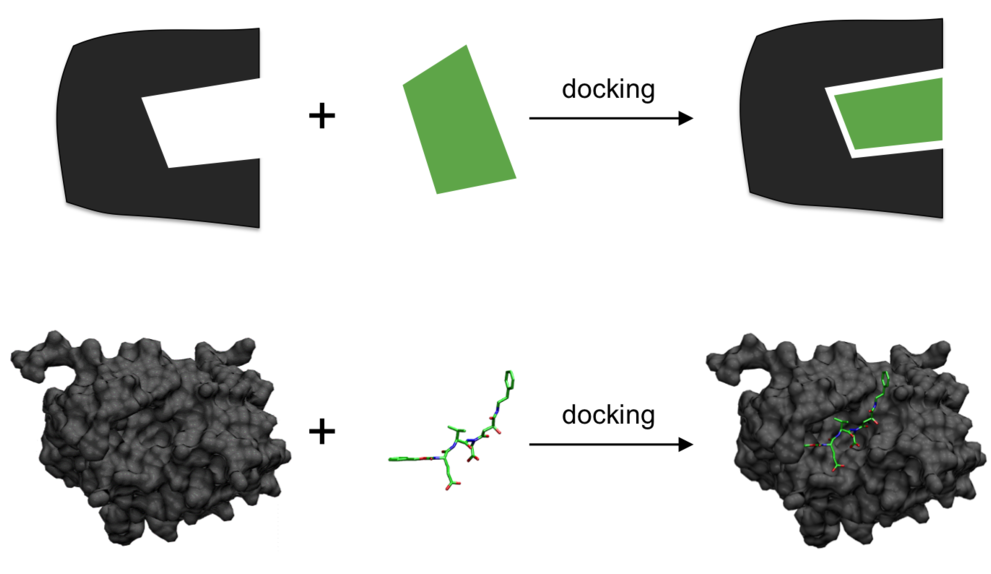
\includegraphics[width=.9\linewidth]{images/docking.png}
\end{center}
\end{block}
\end{frame}
\begin{frame}[label={sec:orgfb815a2}]{Pasos del docking}
\begin{center}
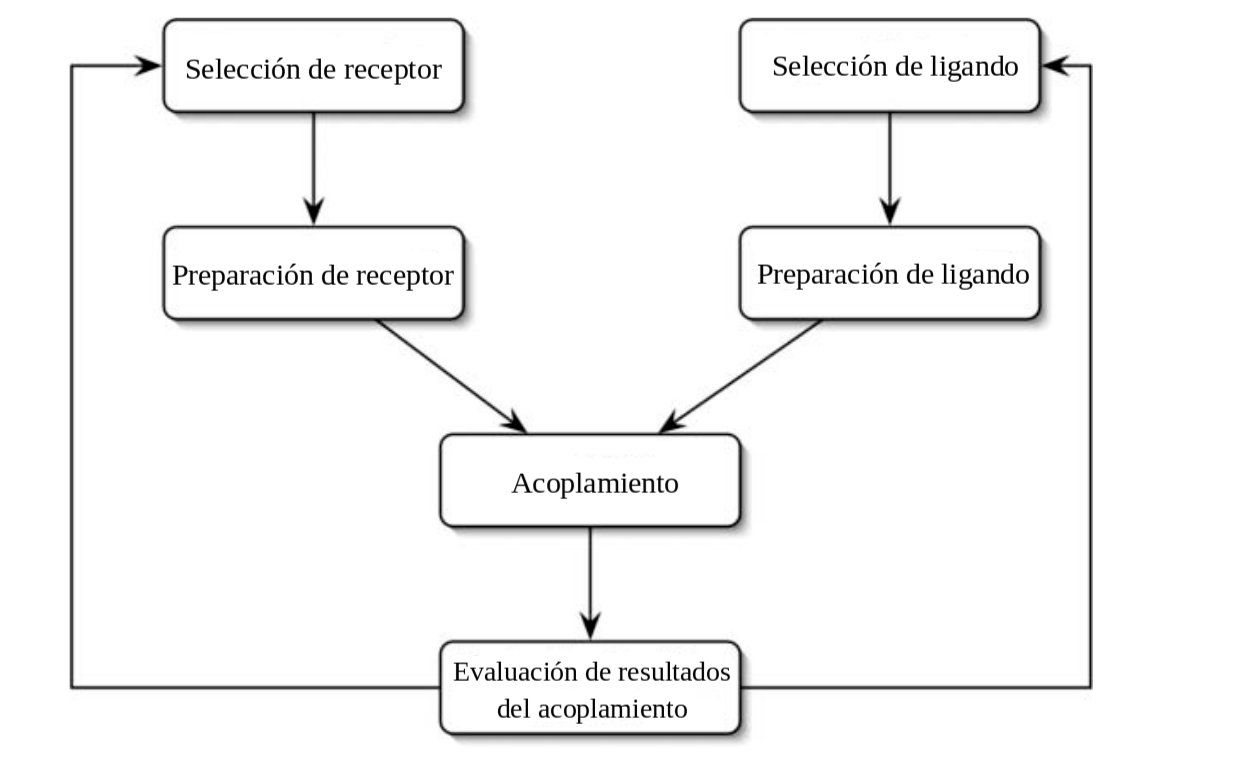
\includegraphics[width=.9\linewidth]{images/docking_steps.png}
\end{center}
\end{frame}
\section{Sobre inteligencia artificial}
\label{sec:orge6ee10c}
\begin{frame}[label={sec:org0a01b6b}]{La prueba de Turing}
\begin{center}
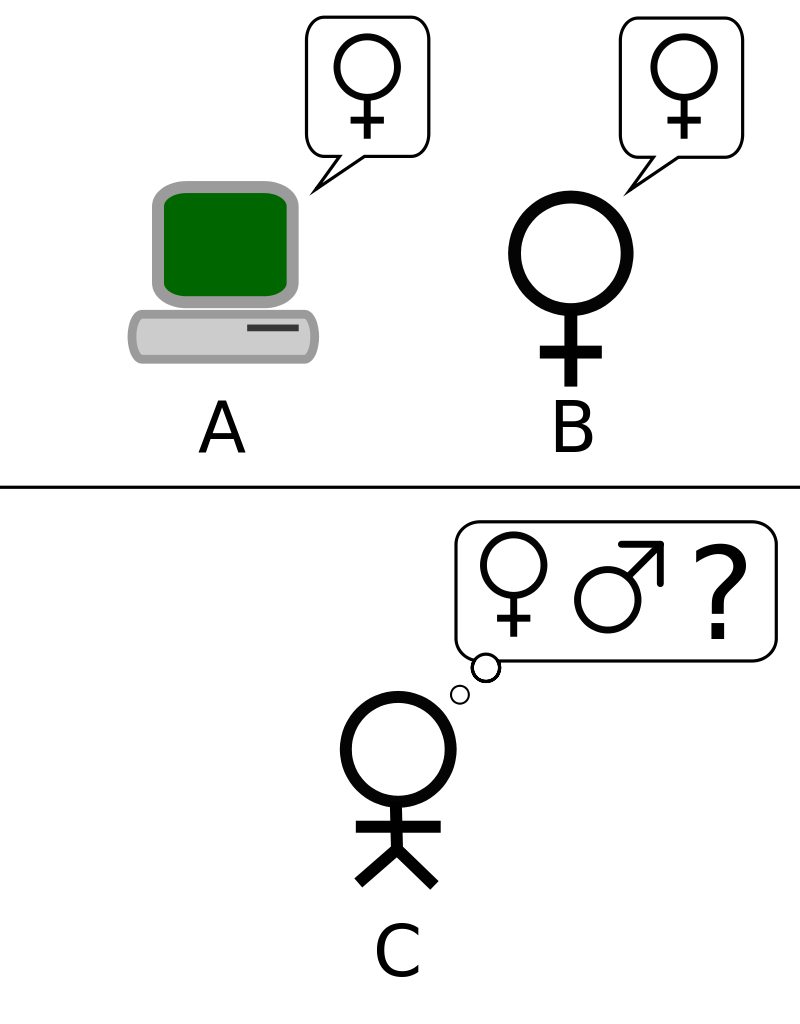
\includegraphics[width=170px]{images/turing-test.png}
\end{center}
\end{frame}
\begin{frame}[label={sec:org100f089}]{IA y agentes}
\begin{block}{Inteligencia artrificial}
\alert{\alert{Agentes racionales}} que, mediante \alert{\alert{sensores}}, pueden
percibir su \alert{\alert{entorno}} y actuar sobre él a partir de un
sistema de decisión.
\pause
\end{block}
\begin{block}{Agentes}
Máquina compuesta por un conjunto finito de estados, cuyas
transiciones están dadas por reglas de inferencias.
\end{block}
\end{frame}
\section{Sobre redes y neurona}
\label{sec:orgd2992d0}
\begin{frame}[label={sec:org9382281}]{Inspiración en la biología}
\begin{center}
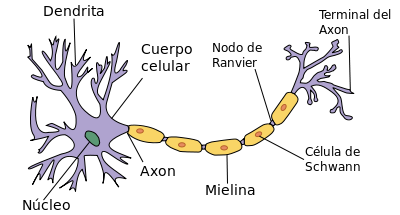
\includegraphics[width=.9\linewidth]{images/neurona.png}
\end{center}
\end{frame}

\begin{frame}[label={sec:org7f252a2}]{Perceptrón}
\begin{block}{Dados asdfasdf}
asdasdfasdf asdfasd iqieid
\end{block}
\end{frame}
\end{document}
